\chapter{Signal Interface}
\mylabel{signals}

The signal interface to the \eco consists of three sets of signals:
\begin{itemize}
\item system operation signals: clock and reset
\item SoC bus signals
\item interrupt signals
\end{itemize}

\begin{figure}[h]
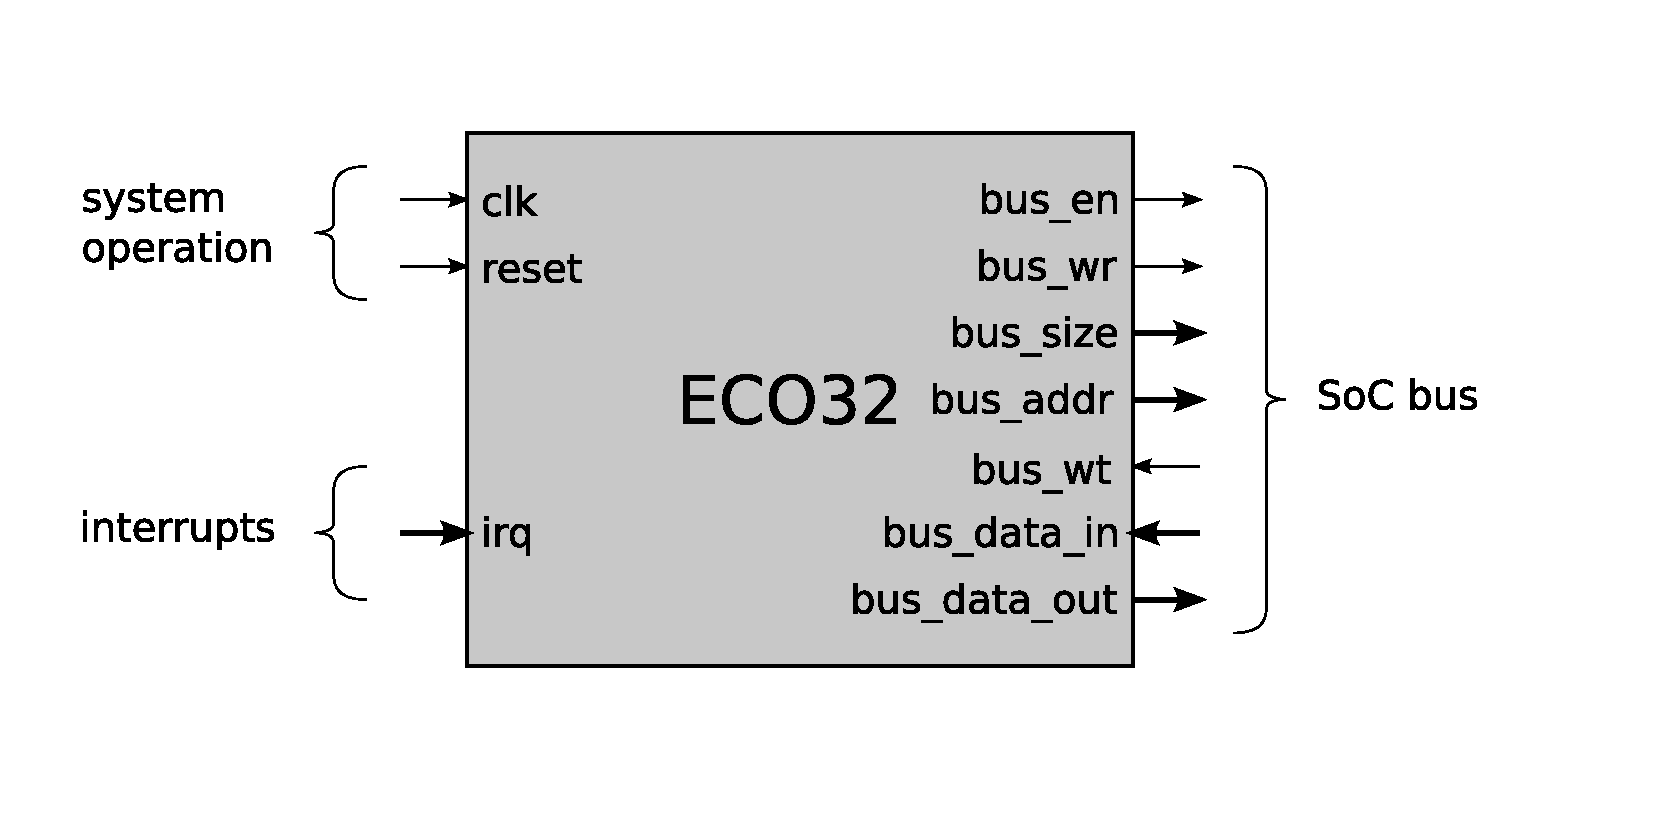
\includegraphics[scale=0.4]{./signals.pdf}
\caption{ECO32 Signal Interface}
\end{figure}

\section{System Operation Signals}
\mylabel{clkreset}

Two system operation signals control the \ecox:
\begin{itemize}
\item The \definition{clk} signal is a positive edge triggered clock signal that controls the timing of the \ecox. Since the \eco is a soft-core processor, minimum and maximum clock frequencies depend on the implementation in an FPGA and cannot be specified in general. The design of the \eco does not impose any particular constraints on the clock frequencies.

All other signals are synchronous to the \name{clk} signal.

\item The \definition{reset} signal is a positive level triggered clock-synchronous reset signal. If the reset is asserted, the \eco is placed into a partly defined reset state, as described in \myref{2}{reset_state} and execution is suspended until the reset is de-asserted. The \eco acts as an inactive master device with respect to the bus interface as long as the reset is asserted.
\end{itemize}

\section{Bus Architecture}
\mylabel{bus}

The \eco can be connected to on-chip devices such as a RAM controller and other devices using a simple SoC bus architecture. The bus uses a synchronous handshake protocol with 32 address bits, 32 data bits, and byte-sized, half-word sized, or word-sized transfers.

Bus operation is divided into \definition{bus cycles}. Each cycle guides a single transfer of a byte, half-word, or word value to or from the \ecox. All transfers are initiated by the \eco and responded to by other devices on the bus. For each transfer, the \eco emits an address that selects both a target device and a location inside that device. It also emits a signal that indicates whether it attempts to read data from that location, or write data to that location. It further emits a signal that indicates the transfer size. Finally, for write operations, the \eco also emits the data to write.

A bus request is responded to by a device with a signal that indicates success of the transfer. If the operation is a read operation, this signal also marks availability of the transferred data. If a certain amount of time passes without any device responding to the request, the transfer is considered failed, and a \name{Bus Timeout Fault} occurs.

\subsection{Bus Timing}

The operation of the SoC bus is synchronous with respect to the system clock. The bus architecture allows to complete a bus cycle with every clock cycle. Peripheral devices may slow down bus operation if they cannot respond fast enough.

A bus cycle begins by the \eco asserting the {\it bus\_en} signal to indicate the start of a transfer. At the same time, it emits the desired values on the {\it bus\_wr}, {\it bus\_size}, {\it bus\_addr}, and {\it bus\_data\_out} lines. The {\it bus\_wr} indicates a read cycle (if de-asserted) or a write cycle (if asserted). The {\it bus\_size} indicates the transfer size, with 10 or 11 indicating a word transfer, 01 indicating a half-word transfer, and 00 indicating a byte transfer. The {\it bus\_addr} is a 32-bit address signal group that selects both a peripheral device and a location in that device. Finally, {\it bus\_data\_out} indicates the transferred data in a write cycle. It is ignored in read cycles. All these signals must keep their value until the clock edge that marks the end of the bus cycle (see below).

The addressed device responds immediately, that is, in the same clock cycle in which the \eco asserted the bus request signals (with no intermediate clock edge), by placing a value on the {\it bus\_wt} line. Each positive clock edge that occurs while {\it bus\_wt} is asserted indicates a wait clock cycle and does not indicate the end of the bus cycle. This allows slower devices to perform internal operations. The device de-asserts {\it bus\_wt} as soon as its internal operations are finished. As soon as a positive clock edge occurs while {\it bus\_wt} is de-asserted, the bus cycle is finished. For read operations, the target device must assert the data to transfer prior to that clock edge, and keep it stable until after that clock edge. The clock cycle following that clock edge is no longer part of the bus cycle, and may witness the start of another bus cycle. Therefore, if the addressed device never asserts its {\it bus\_wt} signal, one bus cycle can be completed in each clock cycle.

If a physical address is emitted on the {\it bus\_addr} lines that is not associated with any device, then the bus itself keeps the {\it bus\_wt} line asserted permanently. This eventually causes the \eco to trigger a \name{Bus Timeout Fault} and stop the bus cycle. A bus timeout is the only event that stops a bus cycle abnormally.

\subsection{Bus Address Map}

The bus architecture places certain restriction on the mapping of physical addresses on the {\it bus\_addr} lines and addresses devices:
\begin{itemize}
\item Addresses in the range 0x00000000 through 0x1FFFFFFF are always associated with a RAM controller. However, only a subrange of these addresses are responded to if the RAM is smaller than 512 MB. RAM may be accessed with (aligned) word, half-word, or byte transfers.
\item Addresses in the range 0x20000000 through 0x2FFFFFFF are always associated with a ROM controller. However, only a subrange of these addresses are responded to if the ROM is smaller than 256 MB. ROM may be accessed with (aligned) word, half-word, or byte transfers.
\item Addresses in the range 0x30000000 through 0x3FFFFFFF are associated with peripheral devices. Their meaning is not further specified. Peripheral device addresses may only be accessed with aligned word transfers.
\item Addresses in the range 0x40000000 through 0xFFFFFFFF are not used. Accesses to these locations will not be responded by any device and cause a \name{Bus Timeout Fault}.
\end{itemize}

\subsection{Bus Sizing}

The {\it bus\_size} signal indicates whether a bus cycle guides a word, half-word, or byte transfer. Access to devices other than RAM or ROM is restricted to word transfers. Half-word and byte transfers on such devices have an unspecified effect.

All word transfers must be aligned to word locations, that is, the lowest two bits of {\it bus\_addr} must be 0. Similarly, half-word transfers must be aligned to half-word locations, that is, the lowest bit of {\it bus\_addr} must be 0. The effect of unaligned transfers is unspecified from the perspective of the SoC bus. The \eco itself prevents such transfers internally and triggers an \name{Illegal Address Fault} instead.

For RAM or ROM locations, a word transfer to or from address $4n$ affects the byte locations $4n$ through $4n+3$ in a big-endian fashion. Similarly, a half-word transfer to or from address $2n$ affects the byte locations $2n$ and $2n+1$ in a big-endian fashion. Write operations change only the affected RAM locations; all other locations are left alone.

During a word transfer, all 32 data lines carry data. During a half-word transfer, only the lower 16 data lines carry transferred data; the others carry unspecified values. During a byte transfer, only the lowest 8 data lines carry data; the others carry unspecified values. Read operations fill the unspecified bits by zero-extending or sign-extending the transferred value. Write operations are either word-sized (in which case there are no unspecified bits), or affect RAM (in which case only 2 or 1 RAM bytes are affected, and the unspecified data lines are ignored).

\subsection{Address Decoding}

During the clock cycle in which the \eco emits a transfer request, the bus decodes addresses by comparing the address sent by the \eco with an individual bit pattern for each device. These patterns are chosen in such a way that at most one comparison succeeds. The corresponding device is \definition{selected} by that address. If no device is selected, the bus asserts the {\it bus\_wt} signal until the \eco detects a timeout.

If a device has been selected, the enable signal for that device is asserted. Thus, the selected device knows it takes part in a transfer by its enable signal. All other devices do not see their enable signal asserted, and thus do not react. A device whose enable signal is de-asserted cannot tell whether a bus transfer involving another device is currently happening.

Since devices whose enable signal is de-asserted do not react to a bus cycle, the bus can safely send the {\it bus\_wr}, {\it bus\_addr}, and {\it bus\_data\_out} to all devices. Devices which have not been selected ignore these values. The same holds true for {\it bus\_size}, but this signal is delivered only to RAM and ROM. All other devices cannot take part in a half-word or byte sized transfer, and implicitly assume word-sized transfers.

Incoming signals from devices are multiplexed by the decoded address. That is, the {\it bus\_wt} and {\it bus\_data\_in} signals arriving at the \eco are those of the selected device. If no device has been selected, {\it bus\_wt} is permanently asserted, and {\it bus\_data\_in} contains a dummy value.

The address lines arriving at each device are a subset of the {\it bus\_addr}. These address lines deliver the \definition{device-local} address. Since each device reacts only if selected, and devices are selected if the address matches a certain bit pattern, only those bits must be delivered that are not yet known by the pattern. Furthermore, delivering those known address bits makes the device unnecessarily sensitive to the positon of its address range in the physical memory map, and thus prevents moving the device to another address range.

The bus may omit further address lines if the corresponding device would ignore them. Most devices need only a tiny subset of their allocated address space, and thus only a subset of the device-local address lines. For example, if the bus uses 12 decoded bits to recognize a device as selected, then that device gets 18 device-local address lines (the lowest two lines are not routed because only aligned word-sized access is allowed). However, a typical device using $8=2^3$ registers would need only 3 device-local address lines. It could then decode the remaining lines and expect them to be 0 (leaving a huge hole in the address map), or ignore them and effectively mirror the 8 registers numerous times to fill the address map. The latter approach requires less hardware resources. However, ignored signal lines usually cause hardware synthesis tools to print warning messages, even if they are bogus as in this case. To prevent these warning messages, the bus may be built such that it does not route the ignored address signals to the device.

By the same reasoning, ignored data signals or other signals can be omitted.

\section{Interrupt Signals}
\mylabel{irqsignals}

The \eco supports 16 interrupt signals that (if accepted) cause a control transfer to the general exception service routine (see \myref{2}{service_routine_address}) and disable interrupt admission temporarily. The interrupt signals need not be associated with other devices on the SoC bus, although this is often the case. The interrupt signals are synchronous, positive level-triggered signals.

Admission of an interrupt is not signalled to the interrupt source automatically. The interrupt service routine must take appropriate action on the SoC bus to cause the corresponding device to de-assert the interrupt signal. Otherwise, as soon as interrupts are enabled again in the \pswx, the still-active interrupt line is recognized again and another interrupt is accepted.

If an asserted interrupt is not immediately accepted by the \eco (e.g. because interrupts are disabled in the \pswx), then the corresponding device can either keep the interrupt signal asserted and be served as soon as the \eco is ready, or de-assert the interrupt signal before the \eco accepts the interrupt and remain unnoticed.
